% Preamble
\documentclass[11pt, oneside]{article}   	%standardeinstellung
\usepackage{amsmath}				%damit du formeln eingeben kannst
\usepackage[parfill]{parskip}    			% neuer absatz durch leere zeile
\usepackage{graphicx}				% bilder einfügen
\usepackage[onehalfspacing]{setspace}	%1,5 facher zeilenabstand
\usepackage{hyperref}				%damit man links erstellen kann
\usepackage{float}					%intelligentes anpassen von bildern, damit es keine lücken im text gibt
\graphicspath{ {figures/} }				%automatisches erstellen von "List of Figures"
\usepackage[font=small,labelfont=bf]{caption} %formatierung der bildunterschrift
 \usepackage{geometry}				%Seitenlayout
 \usepackage{tikz}
 \usetikzlibrary{shapes,arrows}

 \geometry{						%musst du nicht unbedingt selbst einstellen
 a4paper,
 total={210mm,297mm},
 left=15mm,
 right=15mm,
 top=25mm,
 bottom=20mm,
 }

\usepackage{ragged2e}
\usepackage[export]{adjustbox}
\usepackage{dsfont}
\usepackage{amssymb}
\usepackage{caption}
\usepackage{natbib}
\usepackage[utf8]{inputenc}
\usepackage{amsmath}
\usepackage{amsfonts}
\usepackage{amssymb}
\usepackage{wrapfig}
\usepackage{subcaption}
\usepackage{pdflscape}
\usepackage{filecontents,url}
\usepackage{soul}
\usepackage[space]{grffile}
\usepackage[UKenglish]{isodate}

%\def\checkmark{\tikz\fill[scale=0.4](0,.35) -- (.25,0) -- (1,.7) -- (.25,.15) -- cycle;}

\title{Inefficient African Trade Networks}
\author{Tilman Graff -- University of Oxford}
\date{\today}

\begin{document}

\bibliographystyle{cantoni_copy}
\maketitle

% End Preamble

%-------------------------------------------------

\section{Introduction}

\section{The \cite{fajgelbaum_optimal_2017} model of Optimal Transport Networks}

% Chapter
\section{Towards a spatial measure of network inefficiency}

Investigating the patterns behind the spatial distribution of network inefficiency involves a series of steps. First, I construct a representation of the topography of economic activity and infrastructure networks for every African country. Using the model by \cite{fajgelbaum_optimal_2017} outlined above, I then conduct an optimisation exercise in which existing infrastructure is reallocated within each country to maximise overall welfare. This scenario will produce winners and losers, such that I can derive a measure of network inefficiency over regions by comparing current welfare with welfare under the optimised scenario.

Below, I discuss these steps in more detail.

\subsection{Data Sources}

To construct a network database of all African countries, I divide the entire continent into grid cells of 0.5 degrees latitude by 0.5 degrees longitude (roughly 55 by 55 kilometres at the equator). For all of Africa, this amounts to 10,167 cells. Using GIS, I locate the geometric centroid of each cell and overlap these points with current political borders to assign countries to each centroid.\footnote{Data on African borders come from \cite{Sandvik_WorldBordersDataset_2008}. Because of its relative age this dataset does not include borders on South Sudan. I hence add the world's youngest country manually using data from \cite{OCHA_SouthSudanAdministrative_2017}. Taking the centroid position as the decisive statistic to assign countries might lead to situations where cells near oddly shaped borders are assigned country A, even if they mostly lie in country B. However, I don't believe this to be a major concern, especially since colonial legacies have led to African borders being drawn in a particularly straight-line fashion \citep[see][]{Alesina_ArtificialStates_2011}.} I then use spatial data on economic and geographic characteristics from a variety of sources and aggregate them onto the grid cell level.

Raster data on 2015 population totals comes from the \cite{socioeconomic_data_and_applications_center_gridded_2016} and is available on a much finer resolution than the one of my study. I hence aggregate them onto the grid cell level to obtain the total number of people living in each grid cell. On average, a cell is home to 110,000 people, with the median much to the left of that (25,000). The most populous cell contains Cairo and inhabits almost 18 million people. 212 cells are uninhabited.

Geographic characteristics include altitude, soil quality, weather data, malaria prevalence, and terrain ruggedness.\footnote{Note that this version of the indicator slightly improves upon the original quantification of terrain ruggedness in the work by \cite{nunn_ruggedness:_2012}. } These data come from \cite{henderson_global_2018} and are also aggregated to the slightly coarser resolution of my study. \citeauthor{henderson_global_2018} show that these indicators account for a substantial part of the global variation of economic activity and hence serve as an important set of controls for later empirical examinations.

Lastly, to proxy for heterogeneities in economic activity over space, I rely on the established practise of using satellite imagery of light intensity at night. Following the seminal work by \cite{henderson_measuring_2012}, more lit places have been associated with more economic activity or growth in numerous settings, including ethnic homelands \citep{MichalopoulosNationalInstitutionsSubnational2014}, cities \citep{storeygard_farther_2016}, or the Korean peninsula \citep{Lee_InternationalIsolationRegional_2016}.\footnote{See \cite{donaldson_view_2016} for an excellent review.} I use data on night luminosity from \cite{henderson_global_2018} which was captured by satellites in 2010. This dataset bears an improvement over other existing night lights data, as it is able to better discern differences at the very right tail of the light distribution and hence prevents many problems related to top-coding of the highest-lit places. Taking means, this data is also aggregated to the 0.5 x 0.5 degree resolution. Night lights are approximately log-normal distributed and hence have to be converted into logarithmic form when serving as the dependent variable in standard regression settings. However, in the study at hand, lights serve as a calibration parameter for differences in economic output and thus do not have to be transformed.

\subsection{Road Network}
So far, the dataset merely consists of a list of grid cells with their respective characteristics. To gain a conception of their relative position in a trade network, a measure of connectedness between locations is needed. In particular, one needs to know whether two locations are connected at all, how strong the link between the two already is, how costly it is to improve the link, and how costly it is to trade between the two. Or, in the notation of \cite{fajgelbaum_optimal_2017}, an infrastructure matrix $I_{i,k}$, an infrastructure investment cost parameter $\delta_{i,k}^{I}$, and a trade cost parameter $\delta_{i,k}^{\tau}$.

\subsubsection{Road Data}
Obtaining objective data on transportation networks is difficult, especially in developing countries where many transport routes are not available in digitised form. In their own empirical exercise \citeauthor{fajgelbaum_optimal_2017} observe European countries and make use of a large coherent dataset on position and objective characteristics of important European roads. A comparable dataset for Africa does not yet publicly exist, even though a recent project by \cite{jedwab_average_2017} has undertaken the effort to manually compile and digitise Michelin Maps in order to create a comparable dataset (their data is not yet available for replication).

Instead, I use a different approach and make use of the open source internet routing service \textsc{Open Street Maps} (OSM), which is comparable to Google Maps but allows for unlimited use of its API. For every centroid location, I scrape OSM for the optimal route to their respective eight surrounding neighbours. This is greatly facilitated by the R package \texttt{osrmRoute}.\footnote{Calculations were performed in November 2017.} Since I am interested solely in within-country transport networks, I perform the exercise for each country separately and do not elicit connections between locations of different countries. Hence, centroids located near a coast or country border often have less than eight immediate neighbours. For all of the resulting almost 90,000 routes, I gather distance travelled, average speed, and step-by-step coordinates of the travel path.

% Figure
\begin{figure}[t]
\centering
\caption{Road Networks for different countries as scraped off OSM}

\begin{subfigure}[c]{0.48\textwidth}
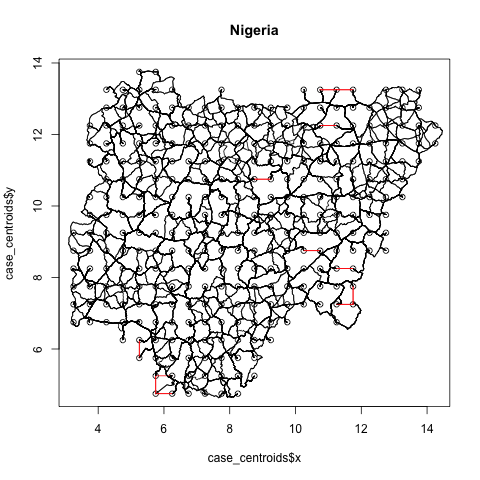
\includegraphics[width=\textwidth]{/Users/Tilmanski/Documents/UNI/MPhil/Second Year/Thesis_Git/Build/output/Road_Networks/network_Nigeria.png}
\caption{Nigeria}
\label{fig:nigeria_roads}
\end{subfigure}
\begin{subfigure}[c]{0.48\textwidth}
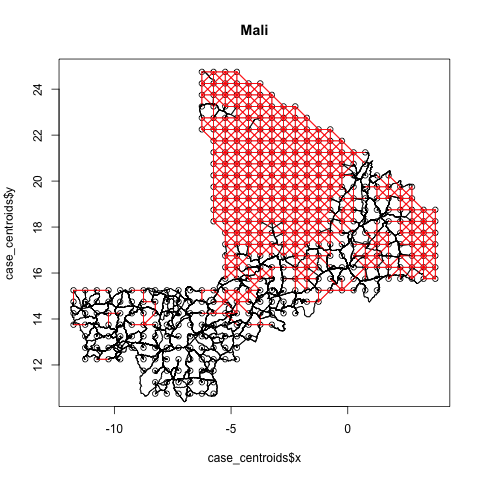
\includegraphics[width=\textwidth]{/Users/Tilmanski/Documents/UNI/MPhil/Second Year/Thesis_Git/Build/output/Road_Networks/network_Mali.png}
\caption{Mali}
\label{fig:Mali_roads}
\end{subfigure}
\label{fig:roads}
\end{figure}
% End Figure

The OSM routing algorithm is specified for cars and takes into account differential speeds attainable on different types of roads. However, if either start or destination location do not directly fall onto a street, the optimal route jumps to the nearest road and goes from there. To take this into account, I add a walking distance to the travel path. Agents are assumed to walk in straight lines to the nearest street at a fixed speed of 4 km/h. They then take the car and drive the route with average speed as specified by OSM, before they potentially have to walk the last stretch again to their exact centroid destination. For some particularly remote areas, the nearest street is very far such that the car routing provided by OSM is not sensible. To counter these cases, I also calculate for all 90,000 connections the outside option of walking the entire link in a straight line at 4 km/h. I then identify cases in which walking directly is actually faster than using OSM's proposed route (plus the travel to and from roads). In these cases, I replace OSM's route with the walking distance and (constant 4 km/h) speed. Figure \ref{fig:roads} presents the resulting road networks for two African countries. Figure \ref{fig:nigeria_roads} displays every optimal route for Nigeria, which appears overall fairly well connected. Commuters mostly seem to be able to drive relatively direct routes between locations, even though cases with substantial detours are also evident at second glance. Connections in which walking were the preferred alternative are displayed in red and fairly rare in Nigeria. Figure \ref{fig:Mali_roads} presents the case of Mali, which paints a different picture: for many connections through the Sahara desert in the North-East of the country, walking straight lines in the sand is actually the fastest way to get from A to B.

%In some rare cases (less than 0.1 per cent of all connections), the OSM algorithm cannot find any route between two neighbouring centroid locations. This mostly is due to an obvious geographic impossibility to connect two nodes. In Guinea-Bissau, for instance one location lies on the Bolama Islands just off the shore of mainland Guinea-Bissau. Its neighbouring locations are all on the mainland and hence unreachable by car. In other cases, both locations to be connected are in deep jungle or swampy regions. In all these cases, I treat the link as if the two locations were not neighbours in the first place. That implies I even forgo the backup possibility of walking the entire distance, with the thought in mind that nobody can walk between islands or through the densest jungle.

Relying on the open source community of OSM does come with some drawbacks. Most importantly, data on the position and quality of roads is user-generated and hence subject to reporting bias. Intuitively, richer areas may appear to be equipped with more roads if local residents have the time and necessary access to a computer to enter their neighbourhoods into the database. As soon as inference is conducted on the relationship between streets and any covariate of development, the resulting estimates will be biased. While this is certainly troubling, I believe this bias to be much more important on finer resolutions than the operating one in this study. Start and destination of the elicited routes are on average more than 55 kilometres apart and travel will hence take place mostly on larger roads and national highways. It is unlikely that these major streets are systematically underreported in OSM, the primary open source routing platform on the Internet, especially compared to the alternative of digitised Michelin maps. Reporting bias will definitely be an issue when trying to find the optimal route \emph{within} a particular small neighbourhood in Accra, but the OSM database should do a fairly good job in finding the optimal route between Accra and Kumasi. It is nevertheless important to keep this potential flaw of the data in mind when conducting inference later on.\footnote{There is a second, less troubling problem with using OSM data. As this study merely pertains to within-country transport networks, I only look at connections between neighbouring locations of the same country. However, in some cases the optimal route between these locations still might go through a neighbouring country. For instance, Senegal is effectively split into two parts by the intersecting country The Gambia. Still, when connecting Senegalese cell centroids just to the north and to the south of The Gambia (which are still less than 60km apart), the route will go over foreign soil. This presents a problem only in later policy recommendations, as political leaders of one country cannot necessarily legislate road improvements abroad. The rest of the analysis is not affected by this issue.}

After having collected data on distance and average speed on the optimal route between all neighbouring centroid locations, the next step is to discretise these data in order to have a tractable network representation capable of performing the trade simulations necessary in the remainder of this study.

\subsubsection{Infrastructure matrix $I_{i,k}$}
To gain a conception of how much two given nodes are connected in the transport network, one needs to derive a numeric measure of how much infrastructure there is on the optimal route between locations. In their own empirical analysis, \cite{fajgelbaum_optimal_2017} have data on the average number on lanes of the streets used on a given route, and whether these streets are national or secondary roads. The OSM algorithm does not supply this detailed level of information for Africa. However, I argue that the authors are only proxying for a much more immediate statistic -- the average speed with which one can travel on a given road. Obviously there are many factors influencing driving speed other than number of lanes or road classifications. Congestion, altitude differences, or potholes come to mind. However, what the authors are trying to capture is an infrastructure investment vehicle to reduce trade costs. Certainly building more lanes on a given road will reduce trade costs. But it will do so by increasing the speed with which cars can travel on that road. I argue that observing the average speed with which transport can occur between two nodes is a much more immediate measure of how well these nodes are connected. I hence propose
\begin{equation}
  I_{i,k} = \textrm{Average Speed}_{i,k}
\end{equation}

This measure is naturally bound from below at 4 km/h, as walking the air-line distance is always available as a backup. Empirically, average speeds range between 6 km/h (Mauritania, where most of the distances through the desert have to be covered by walking) and 33 km/h (Swaziland). It is now the objective of the policymaker or social planner to reduce trade costs between suitable trade partners by increasing the average speed $I_{i,k}$ with which transport can occur between them.

\subsubsection{Infrastructure building cost matrix $\delta_{i,k}^{I}$}
The constraint of the policymaker in this exercise is that increasing $I_{i,k}$ comes at a cost. In particular, building an additional $I_{i,k}$ between locations $i$ and $k$ costs $\delta_{i,k}^{I}$. The total infrastructure budget in the economy is fixed at $K$, such that
\begin{equation}
  \sum_{i}^{}\sum_{k \in N(i)}^{} \delta_{i,k}^{I}I_{i,k} = K
  \label{eq:infr_building_constraint}
\end{equation}

where $N(i)$ denotes the set of surrounding neighbours of node $i$. $\delta_{i,k}^{I}$ depends on a variety of inputs, like the distance of a road or the underlying terrain. I follow \citeauthor{fajgelbaum_optimal_2017} who in turn make use of a recent study by \cite{collier_cost_2015} who estimate infrastructure building costs in the Developing World. Following \citeauthor{fajgelbaum_optimal_2017}, I calculate
\begin{equation}
  \textrm{ln}\Big(\frac{\delta^{I}_{i,k}}{\textrm{dist}_{i,k}}\Big) = \textrm{ln}(\delta_{0}^{I}) - 0.11*(\textrm{dist}_{i,k} > 50km) + 0.12*\textrm{ln}(\textrm{ruggedness}_{i,k})
\end{equation}

Note that every route in my sample is longer than 50 kilometres and the corresponding dummy term is hence always 1. $\delta_{0}^{I}$ is a scaling parameter. Following \citeauthor{fajgelbaum_optimal_2017}, I normalise $K=1$ for every country and thus flexibly alter $\delta_{0}^{I}$ such that equation (\ref{eq:infr_building_constraint}) is satisfied.

\subsubsection{Trade cost parameter $\delta_{i,k}^{\tau}$}
Trade costs between locations are modelled in the standard iceberg formulation, whereby in order for one unit to arrive in destination $k$, precisely $(1+\tau_{i,k})$ units have to leave origin $i$. Perhaps surprisingly, even though trade costs are such an influential concept in the trade literature very few reliable estimates of their magnitude exist. \citeauthor{fajgelbaum_optimal_2017} propose a tractable functional form in which $\tau_{i,k}(Q_{i,k}, I_{i,k})$ depends negatively on the invested infrastructure $I_{i,k}$ (derived above) and positively on goods shipped $Q_{i,k}$ on a given link (a notion they refer to as \emph{congestion}):
\begin{equation}
  \tau_{i,k}(Q_{i,k}, I_{i,k}) = \delta^{\tau}_{j, k} \frac{Q_{i,k}^{\beta}}{I_{i,k}^{\gamma}}
\end{equation}
with $\beta = 1.245$ and $\gamma = 0.5\beta = 0.6225$ ensuring convexity. $\delta^{\tau}_{j, k}$ is a scaling parameter. \citeauthor{fajgelbaum_optimal_2017} calibrate is as a linear function of the distance between $i$ and $k$ and in order to match some particular patterns from Spanish trade data. This calibration is not applicable to the given context. Firstly, it deals with European developed countries which recent evidence suggests face much less stifling trade costs than the African continent \citep[see e.g.][]{Anderson_Tradecosts_2004}. Secondly, their calibration revolves around different measures for economic output $Y_{i}$ and infrastructure investment $I_{i,k}$ and will hence produce arbitrary estimates for $\delta^{\tau}_{j, k}$.

Instead, I make use of the recent contribution by \cite{atkin_whos_2015}. They use barcode-level data on sale prices of identical goods to back out trade costs between regions within two African countries, Nigeria and Ethiopia. They show that trade costs are significantly increasing in distance between origin and destination and estimate the trade cost elasticity to (log) distance as $0.0374$ for Ethiopia and $0.0558$ for Nigeria. Directly using the average of these two point estimates, I calculate
\begin{equation}
  \delta^{\tau}_{i,k} =  0.466*log(\textrm{dist}_{i,k})
\end{equation}

This specification treats $\textrm{dist}_{i,k}$ as fixed. It hence precludes the policy maker from building a completely new road between locations that were until now only connected via an extensive detour. The only possibility on her hand is to make travel along a given route faster, not to design a completely new route. This will prevent the model to conceive new roads that go right through a swamp or big mountain, but instead propose an improvement of the existing road that goes around the mountain.

\subsection{Heterogeneous goods}
To build incentives for trade, I introduce two different goods: an agricultural and an urban good, which are aggregated in canonical CES fashion. Since economic output is proxied by night luminosity, I cannot observe the distribution of different goods in a given grid cell, but only their total production. I hence assume that urban grid cells are solely producing the urban good, while all other grid cells are producing nothing but the agricultural good. This largely follows \citeauthor{fajgelbaum_optimal_2017}, except that they also allow for differentiation even amongst the largest producing cities. For ease of interpretation (and computation), I stay with a two-good economy.

To classify grid cells as urban or rural, I use an iterative procedure which seeks to match each country's 2016 urbanisation rate as reported by \cite{the_world_bank_world_2017}.\footnote{I start by assuming every location is a city and then gradually proceed to re-classify the least densely populated locations, until the ratio of people living in urban areas to total population equals that of the WDI. For three countries, the WDI do not report urbanisation rates. In these cases, I match the overall urbanisation rate for the entire African continent of 42 per cent as reported by \cite{lall_africas_2017}.} With this procedure, 7 per cent of grid cells are classified as urban. These cells inhabit 40 per cent of the continent's population, matching recent figures from \cite{lall_africas_2017} fairly well.

Since labor is fixed, I do not have to impose a strict production function. In fact, the model stays agnostic about how grid cells produce their luminosity output. This is in contrast to \citeauthor{fajgelbaum_optimal_2017} who do allow for endogenous labor allocation across cities and goods and hence need to take a stance on functional forms of total factor productivity and output. The only assumption my model makes is that cells can ever only produce one of the two varieties and hence their productivity in the respective other variety is zero.\footnote{Thanks to this parsimonious specification, I do not rule out the impact of capital or any inputs other than labour to the production function. I also avoid having to divide total lights by total population in order to obtain TFP, a procedure recent literature has explicitly warned against \citep[see e.g.][]{michalopoulos_spatial_2018}.}

\begin{figure}[t]
\centering
\caption{Discretised Networks for different countries}

\begin{subfigure}[c]{0.48\textwidth}
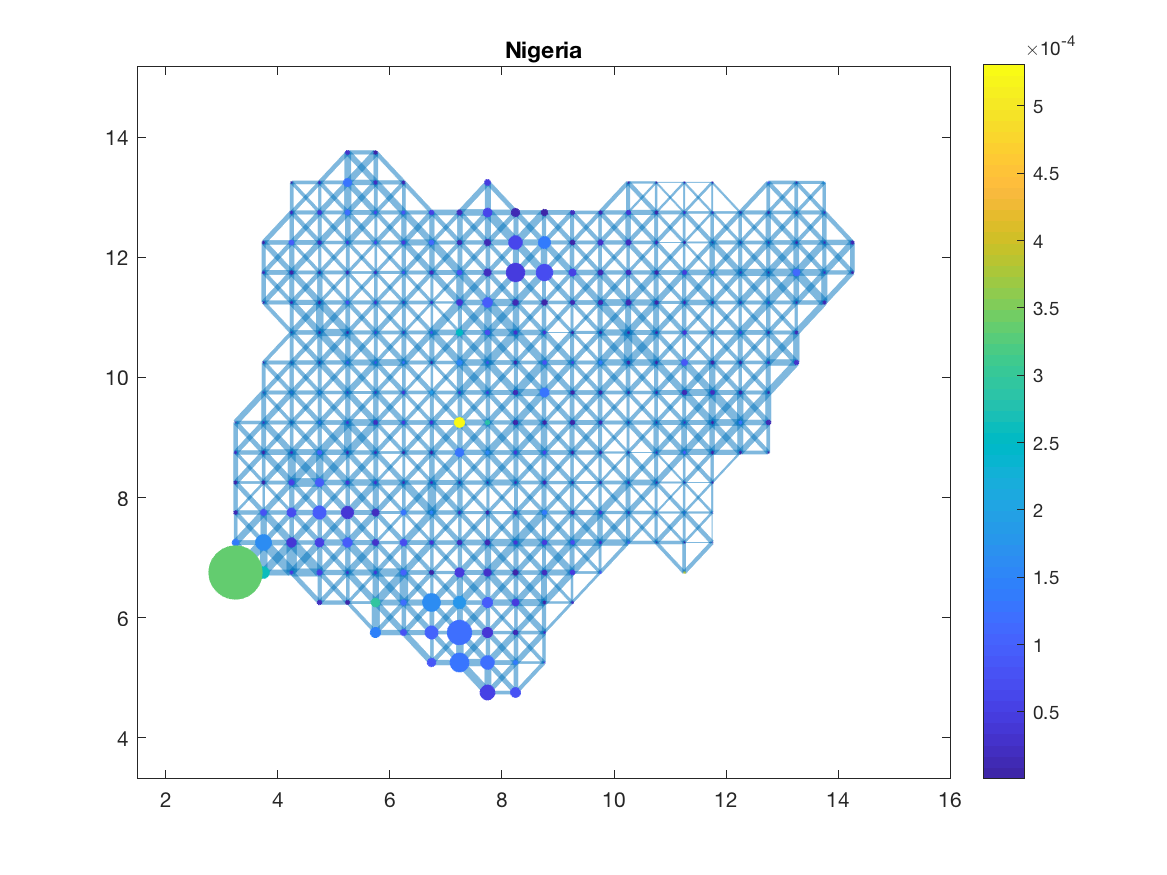
\includegraphics[width=\textwidth]{/Users/Tilmanski/Documents/UNI/MPhil/Second Year/Thesis_Git/Build/output/Matlab_graphs/initial_infrastructure/Nigeria_graph.png}
\caption{Nigeria}
\label{fig:nigeria_mat}
\end{subfigure}
\begin{subfigure}[c]{0.48\textwidth}
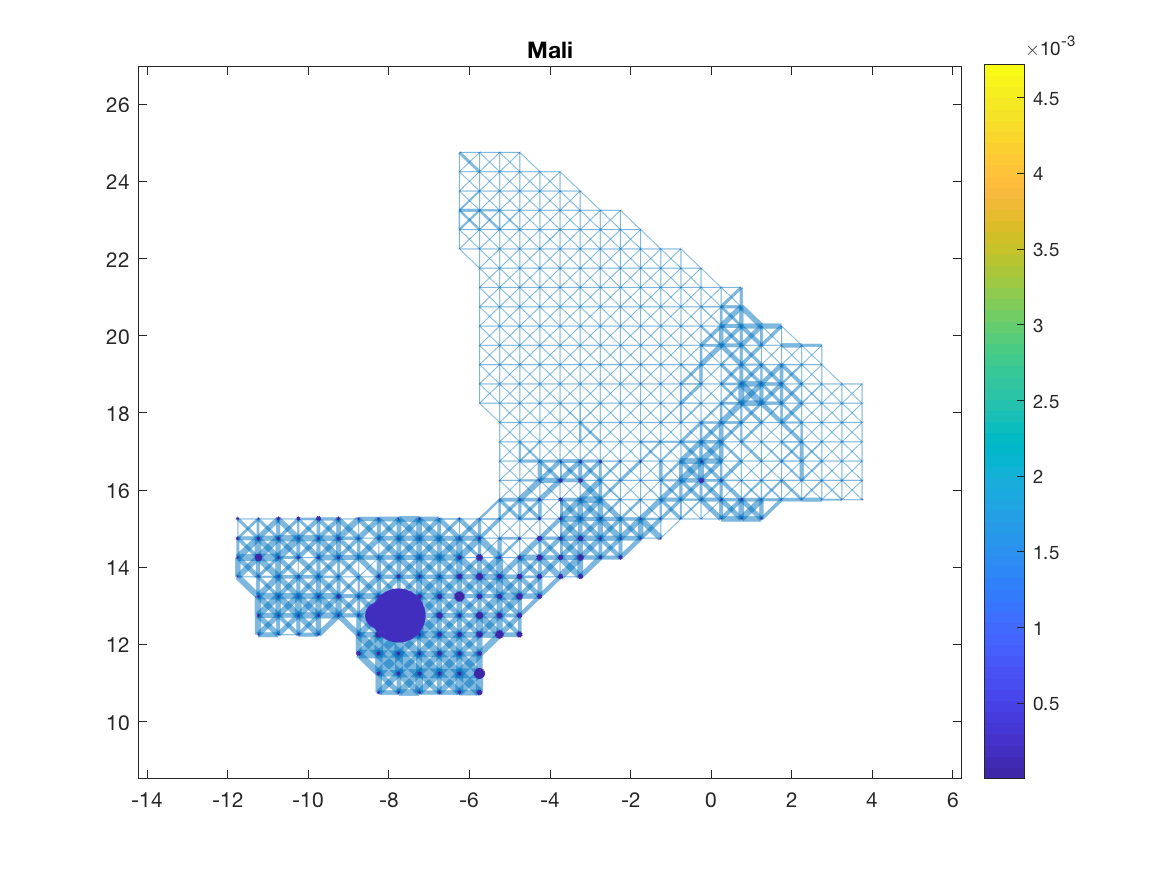
\includegraphics[width=\textwidth]{/Users/Tilmanski/Documents/UNI/MPhil/Second Year/Thesis_Git/Build/output/Matlab_graphs/initial_infrastructure/Mali_graph.png}
\caption{Mali}
\label{fig:Mali_mat}
\end{subfigure}
\label{fig:matlab_networks}
\end{figure}

\subsection{Simulation}

After these steps, a discretised network representation now exists for every African country. Nodes in the network are the spaced centroid locations of each grid cell. They combine the characteristics of the entire grid cell (population, output, etc.) in one point. Edges in the network are road connections between centroids. Each edge carries a number of characteristics (average speed, trade costs, and infrastructure building costs). Figure \ref{fig:matlab_networks} presents this discretised network specification for the two countries from above. Nodes are printed larger proportional to their population. A node's colour scale reflects night light intensity per capita (a statistic which is only calculated for illustrative purposes). Edges are drawn thicker proportional to the initial infrastructure investment (i.e. average attainable speed).

For each country, I proceed to conduct two simulation exercises. In the first, infrastructure $I_{i,k}$ is treated as fixed. This is to obtain a baseline estimate of the spatial variation of welfare in each country. I conduct a social planner exercise whose goal it is to choose trade flows in order to maximise total welfare. This fairly standard static exercise generates the need for trade mostly out of product differentiation. Cities do not produce the agricultural good and hence need to import from surrounding rural backlands, and vice-versa. To facilitate computation and make the problem tractable, \citeauthor{fajgelbaum_optimal_2017} show that instead of optimising over the space of trade flows, the social planner can indeed optimise over the much sparser set of prices. Since strong convexity holds, the solution is unique and a certain price field will induce trade flows and consumption patterns that maximise total welfare. The authors also show how the two welfare theorems hold in this setting and the social planner outcome can hence be supported by a decentralised market solution.

As labor is fixed, the resulting solution will have two properties. Firstly, total output over the entire country will remain untouched. Labour inputs do not shift to more productive regions. Indeed, any welfare gains will be attained solely by shipping the right quantity and mix of goods to the right regions. Second, labor immobility will leave welfare differences between regions as agents cannot simply move to privileged cells. The social planner would like to overcome these differences, but is confronted by trade costs which might leave certain remote areas much worse off than well-connected ones.

Following this static exercise, I proceed to the main task of endogeneising the infrastructure matrix $I_{i,k}$. Intuitively, the social planner is now free to improve connections to a remote area in order to supply them better. \citeauthor{fajgelbaum_optimal_2017}'s main contribution is showing that under particular assumptions, this task can be accomplished simply by means of an additional constraint. Improving on infrastructure yields the benefit of more utility smoothing over space, yet comes at cost $\delta_{i,k}^{I}$. Returns to improving $I_{i,k}$ are not unbounded, however, as the congestion assumption ensures convexity and hence an interior solution to trade flows exists.

To gain a notion of network inefficiency, I run the following scenario: while the social planner is free to manipulate any given link between neighbouring locations, take away or add to existing infrastructure, the total amount of infrastructure in the economy remains fixed. Formally, this corresponds to $K = 1$ in equation \ref{eq:infr_building_constraint} and is what \citeauthor{fajgelbaum_optimal_2017} call the \textit{Optimal Reallocation Scenario}. If the social planner wants to improve the connection between two given locations, she will have to take away infrastructure from somewhere else in the country. The entire exercise does not seek to identify where to place the optimal new investment, but rather represents an utterly fictitious scenario in which every road can be lifted from the ground, reshuffled, and eventually located someplace else.\footnote{Note that equation \ref{eq:infr_building_constraint} only fixes $\sum_{i}^{}\sum_{k \in N(i)}^{} \delta_{i,k}^{I}I_{i,k} = K$. Hence, not the overall sum of infrastructure is fixed, but more precisely the overall cost of infrastructure. This still allows the social planner to take away one unit of infrastructure on a very expensive (high $\delta_{i,k}^{I}$) link and exchange it for much more than one unit on a cheaper (low $\delta_{i,k}^{I}$) link.} This procedure does not measure how many roads a country has, but rather how well they are placed. It does not look at whether the entire country is full of speedy roads, but rather whether those roads connect the right locations.

\begin{figure}
\centering
\caption{Optimal Reallocation Scenario in the Central African Republic}

\begin{subfigure}[c]{0.48\textwidth}
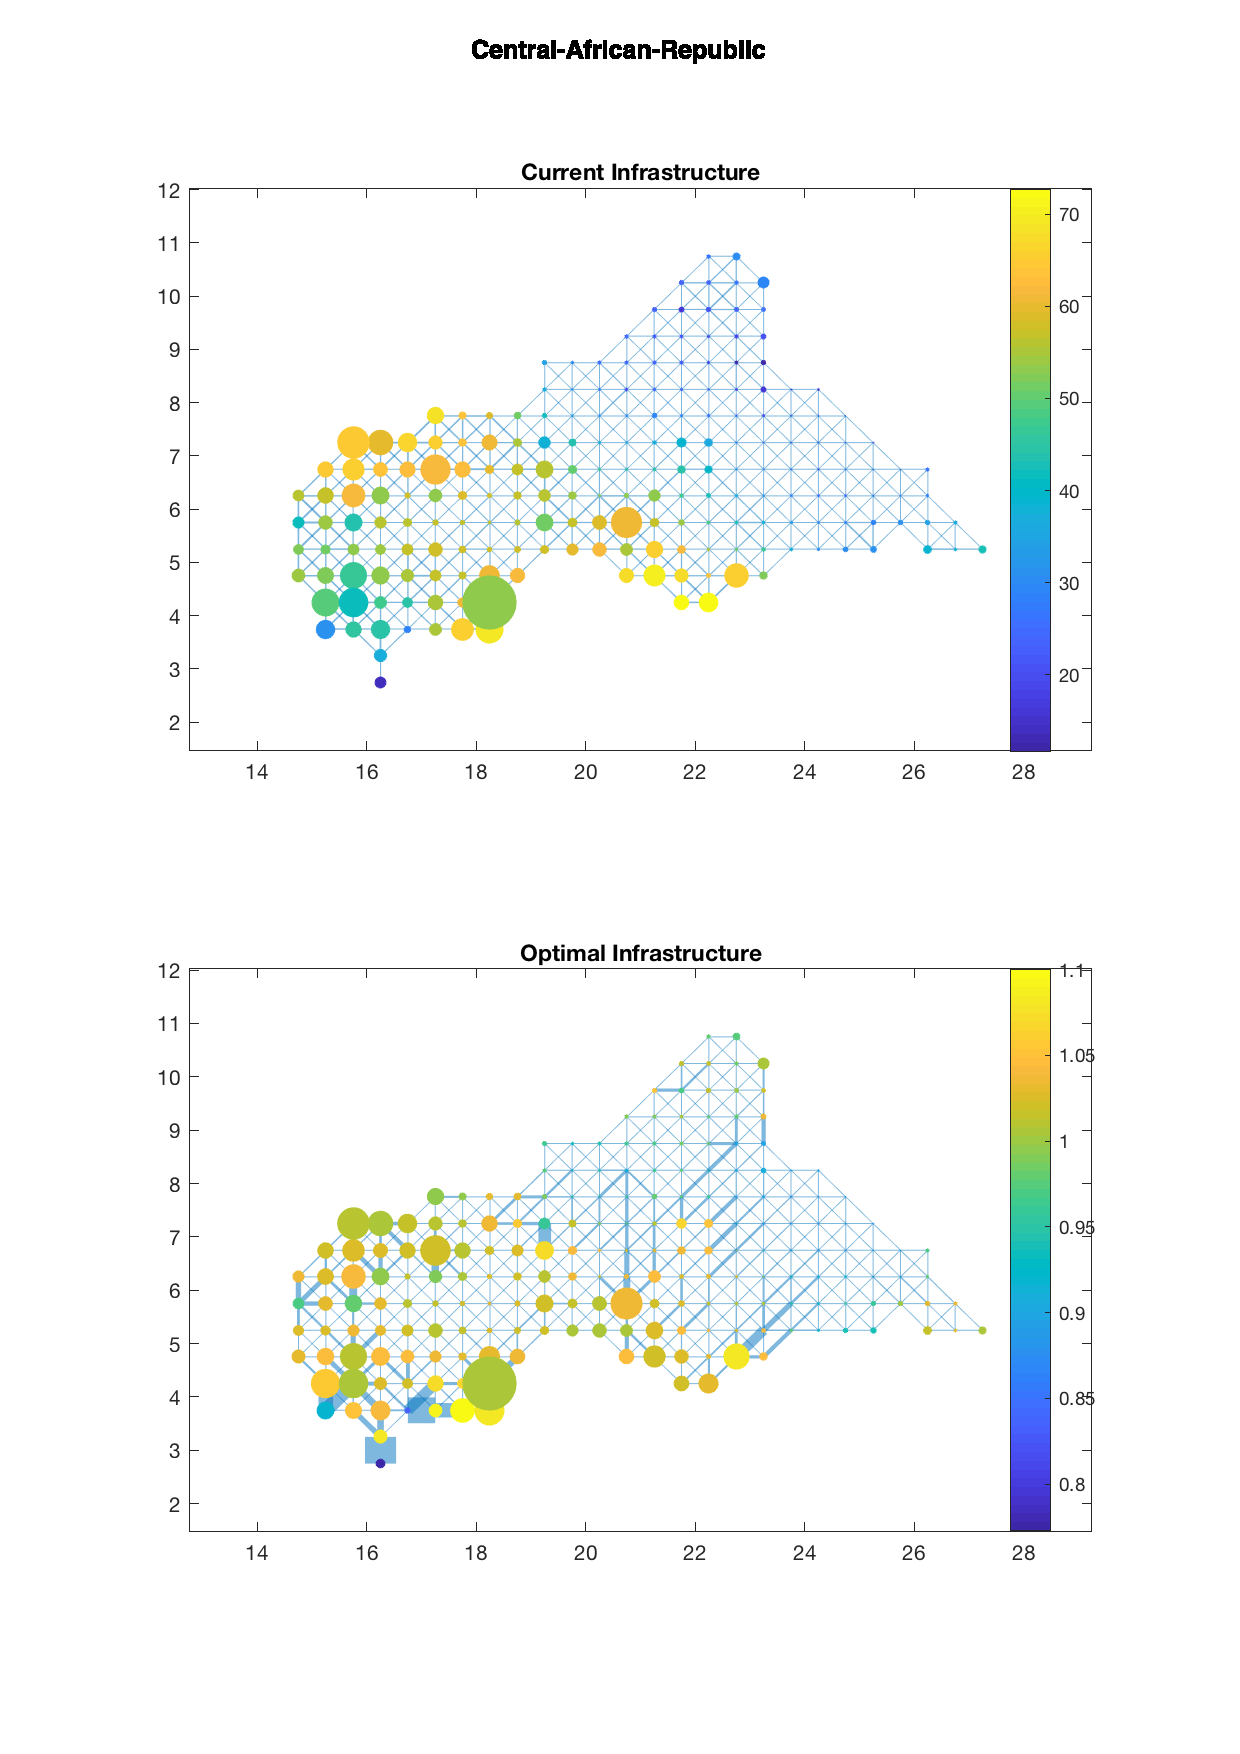
\includegraphics[width=\textwidth,trim={2cm 15cm 2cm 2cm},clip]{/Users/Tilmanski/Documents/UNI/MPhil/Second Year/Thesis_Git/Build/output/Matlab_graphs/optimised_network/Central-African-Republic_graph.pdf}
\caption{Before Reallocation}
\label{fig:before_restructure}
\end{subfigure}
\begin{subfigure}[c]{0.48\textwidth}
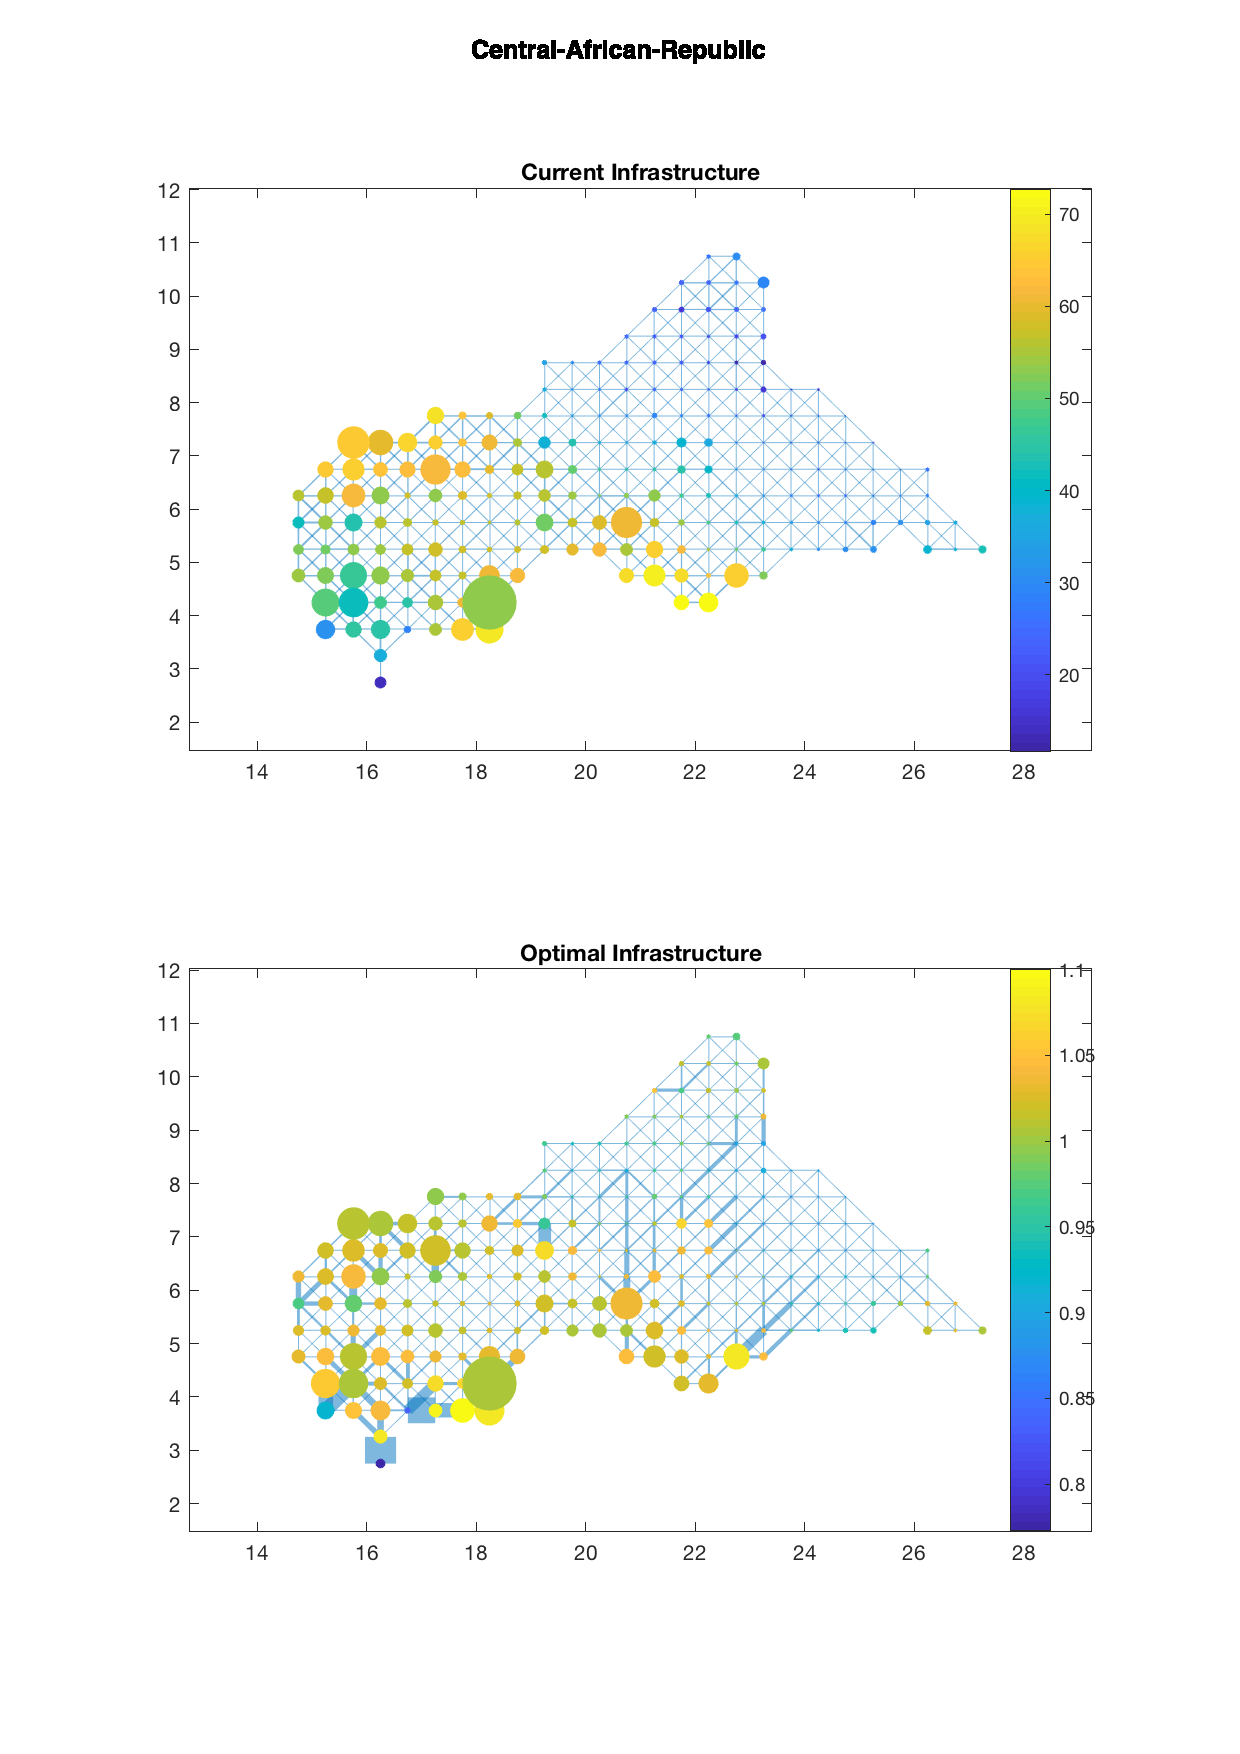
\includegraphics[width=\textwidth,trim={2cm 1.5cm 2cm 15cm},clip]{/Users/Tilmanski/Documents/UNI/MPhil/Second Year/Thesis_Git/Build/output/Matlab_graphs/optimised_network/Central-African-Republic_graph.pdf}
\caption{After Reallocation}
\label{fig:after_restructure}
\end{subfigure}
\label{fig:restructure_centralafricanrepublic}
\end{figure}

Figure \ref{fig:restructure_centralafricanrepublic} visualises this reallocation exercise for the Central African Republic. Subfigure \ref{fig:before_restructure} displays the discretised network representation of the country, comparable to figures \ref{fig:nigeria_mat} and \ref{fig:Mali_mat}. The edges to this network are printed almost evenly thick, implying that infrastructure is fairly evenly distributed across the country. Subfigure \ref{fig:after_restructure} then displays the country after the network reshuffling exercise. Two patterns stand out. First, the social planner sees a heavy need to connect the populous areas in the south west of the country to with more speedy roads. For that, she is willing to salvage some of the unnecessary infrastructure in the middle or north of the country. Second, there still seems to be a benefit from having a few trails connecting the south west with the north east of the country. Some clear north-south and east-west highways spanning multiple regions emerge.

I conduct the reallocation scenario for every African country. Five small countries (Cape Verde, Comoros, The Gambia, Mauritius, and Reunion) are too small to form a sensible network as they only show up as a single location in the dataset and are henceforth no longer considered. Computation times are greatly diminished when exploiting the strong convexity of the optimisation setting and solving the dual problem as outlined in the appendix of \cite{fajgelbaum_optimal_2017}. Optimisations are performed via Matlab's \texttt{fmincon} command. When conducting the simulations, I bound the social planner's set of permissible roads from below, at 4 km/h (such that $I_{i,k} \geq 4$ $ \forall i,k$). This is motivated by the assumption at the beginning that walking straight lines at this speed is conceived as an outside option and always available to any commuter. The social planner should not be able to force commuters to travel slower than walking, in order to build a faster road elsewhere.\footnote{Contrarily, I do not restrict possible investments from above (or at least not in addition to the restriction imposed by equation \ref{eq:infr_building_constraint}), as this could violate the strong convexity of the problem. Not bounding the problem in principle allows the social planner to build supersonic speed highways. However, the model is calibrated in a way that makes this very unattractive to the planner anyway. After simulating reallocation in every African country, less than 0.8\% of all built roads were suggested to be over 260 km/h. Still, one outlier of 2007 km/h (in Egypt) and one of 1755 km/h (in South Africa) remain.}

After successfully reshuffling a country's transport network, overall welfare will necessarily (weakly) increase. It is the social planner's objective to maximise overall welfare, and since the original network composition is always still available, the entire country cannot on aggregate be worse off than before. Note as before that due to labor immobility, overall production (light output) will be the same as before. Welfare gains are solely due to enabling mutual benefits from trade by connecting the right locations. The Central African Republic of figure \ref{fig:restructure_centralafricanrepublic}, for instance, stands to gain 1.84\% of overall welfare just by reshuffling roads. Since this welfare gain is rather hard to materialise, I prefer thinking of it as a measure of network inefficiency. The higher the hypothetical gains from merely reshuffling existing roads, the more haphazard the existing allocation of roads, and hence the more inefficient the current transport network.

\begin{figure}
\centering
\caption{African countries by network inefficiency}
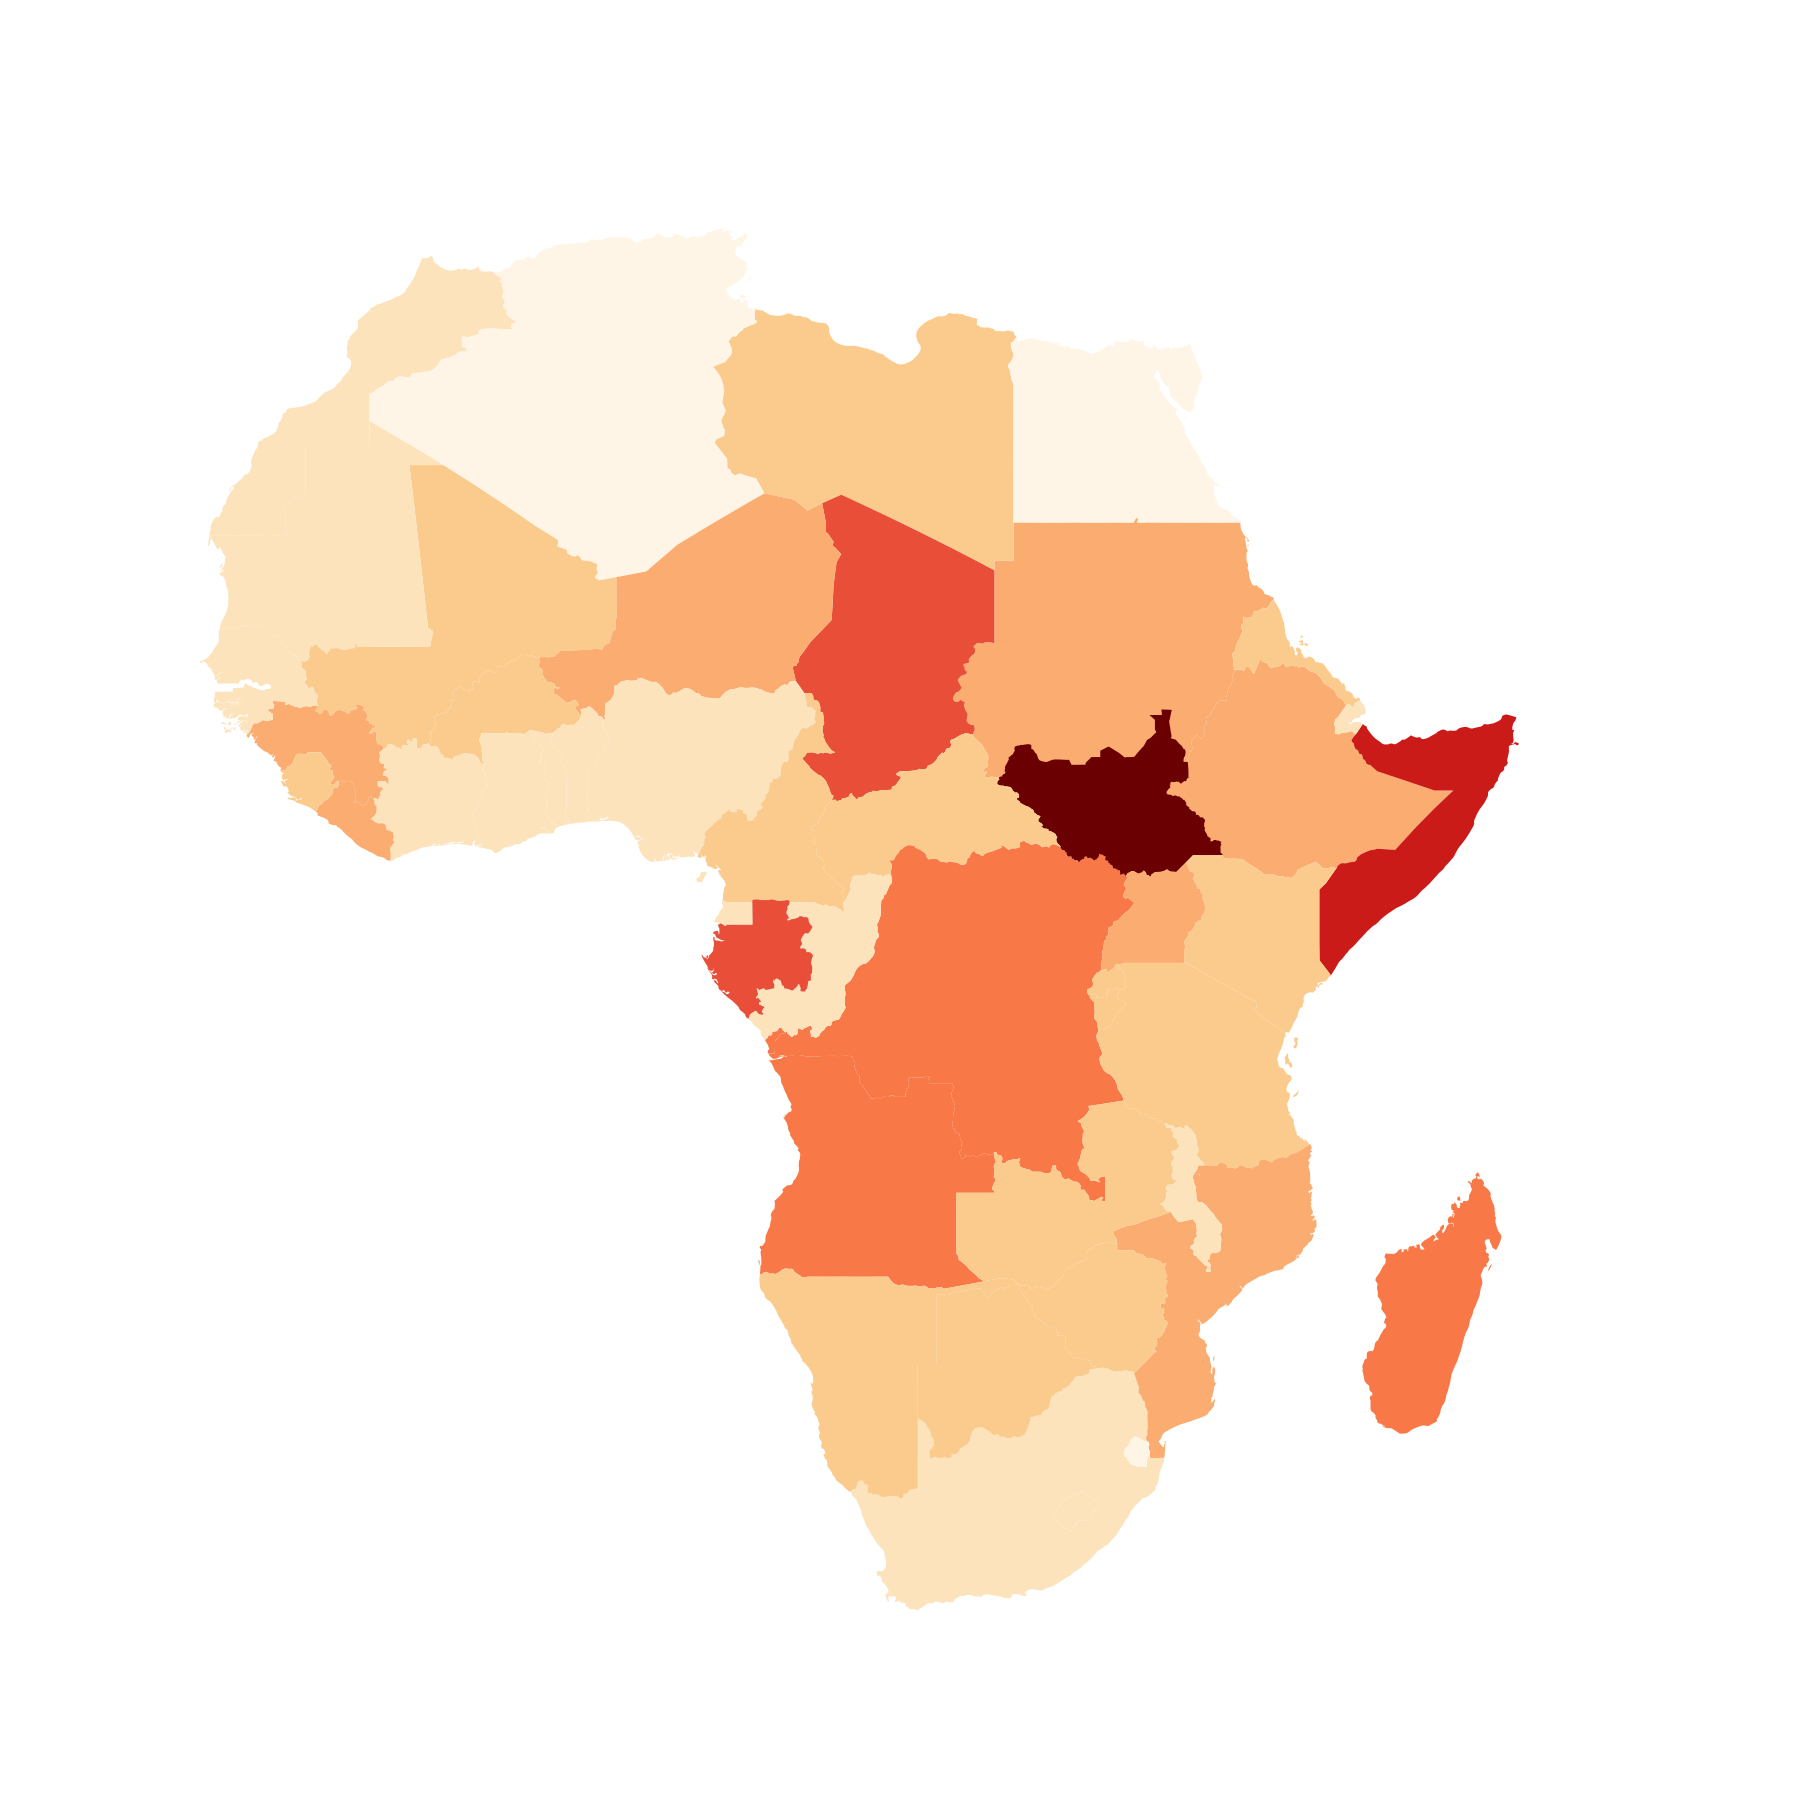
\includegraphics[width=0.6\textwidth]{/Users/Tilmanski/Documents/UNI/MPhil/Second Year/Thesis_Git/Analysis/output/zeta_heatmaps/African_countries_zeta.png}

\label{fig:countries_by_welfare_gain}
\end{figure}

Figure \ref{fig:countries_by_welfare_gain} displays all African countries and their measure of network inefficiency. The closer the forgone welfare gain to zero (the lighter the country's colour), the more efficient the current allocation of roads. The Central African Republic's measure of 1.84\% makes the country look rather good in comparison. Some (mostly more developed) countries like South Africa (0.47\%) or Tunisia (0.24\%) perform even better. Many countries are leaving much more on the table like Somalia (4.76\%) or Chad (4.28\%). No African country, however, has a more ill advised road network than South Sudan (6.66\%). This might not come as a surprise, as the world's youngest country has largely inherited a road network that was not conceived to sustain an independent nation, but connect it to its former capital up north. On a simple cross-country level, more inefficient networks are significantly correlated with more corruption ($p < 0.01$), less property rights ($p < 0.01$) and less 2010 log GDP ($p=0.07$). Note that these are merely descriptive correlations which are far from implying any form of causation.\footnote{Data from \cite{the_world_bank_world_2017}. For corruption and property rights, data is only available for 35 countries and correlations are hence performed on this truncated sample.}

While each country only stands to gain overall welfare from this reallocation procedure, individual locations might very well lose in the process. Intuitively, some regions might be equipped with far too many good roads such that the social planner takes these roads away to use someplace else. Comparing each grid cell's welfare before and after the major reshuffling can help identify regions which are currently over or under-provided for. More formally, I define

\begin{equation}
  \zeta_{i} = \frac{\textrm{Welfare under the optimal Infrastructure}_{i}}{\textrm{Welfare under the current Infrastructure}_{i}}
\end{equation}

% Figure
\begin{figure}
\centering
\caption{Spatial Distribution of $\zeta_{i}$ for sample countries}

\begin{subfigure}[c]{0.32\textwidth}
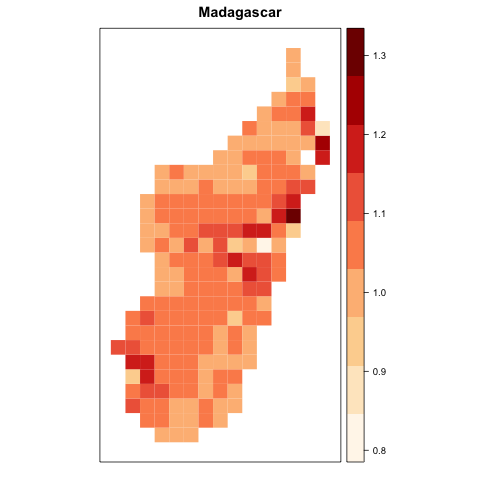
\includegraphics[width=\textwidth]{/Users/Tilmanski/Documents/UNI/MPhil/Second Year/Thesis_Git/Analysis/output/zeta_heatmaps/Madagascar_zeta.png}
\caption{Madagascar}
\label{fig:Madagascar_zeta}
\end{subfigure}
\begin{subfigure}[c]{0.32\textwidth}
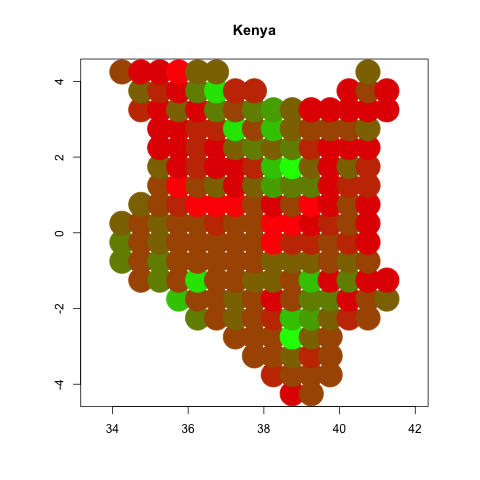
\includegraphics[width=\textwidth]{/Users/Tilmanski/Documents/UNI/MPhil/Second Year/Thesis_Git/Analysis/output/zeta_heatmaps/Kenya_zeta.png}
\caption{Kenya}
\label{fig:Kenya_zeta}
\end{subfigure}
\begin{subfigure}[c]{0.32\textwidth}
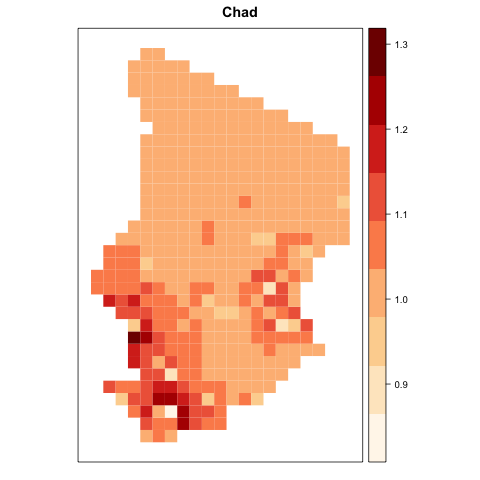
\includegraphics[width=\textwidth]{/Users/Tilmanski/Documents/UNI/MPhil/Second Year/Thesis_Git/Analysis/output/zeta_heatmaps/Chad_zeta.png}
\caption{Chad}
\label{fig:Chad_zeta}
\end{subfigure}
\label{fig:zeta_countries}
\end{figure}
% End Figure

as the \emph{Infrastructure Gap} for each grid cell $i$. Figure \ref{fig:zeta_countries} displays the spatial distribution of the infrastructure gap $\zeta_{i}$ for Madagascar, Kenya, and Chad. The darker a grid cell's shade, the more it is disadvantaged by the inefficiencies of the current network. The lighter a cell, the more overprovided a region is with infrastructure.

% Figure
\begin{figure}
\centering
\caption{Spatial Distribution of $\zeta_{i}$ for entire sample}
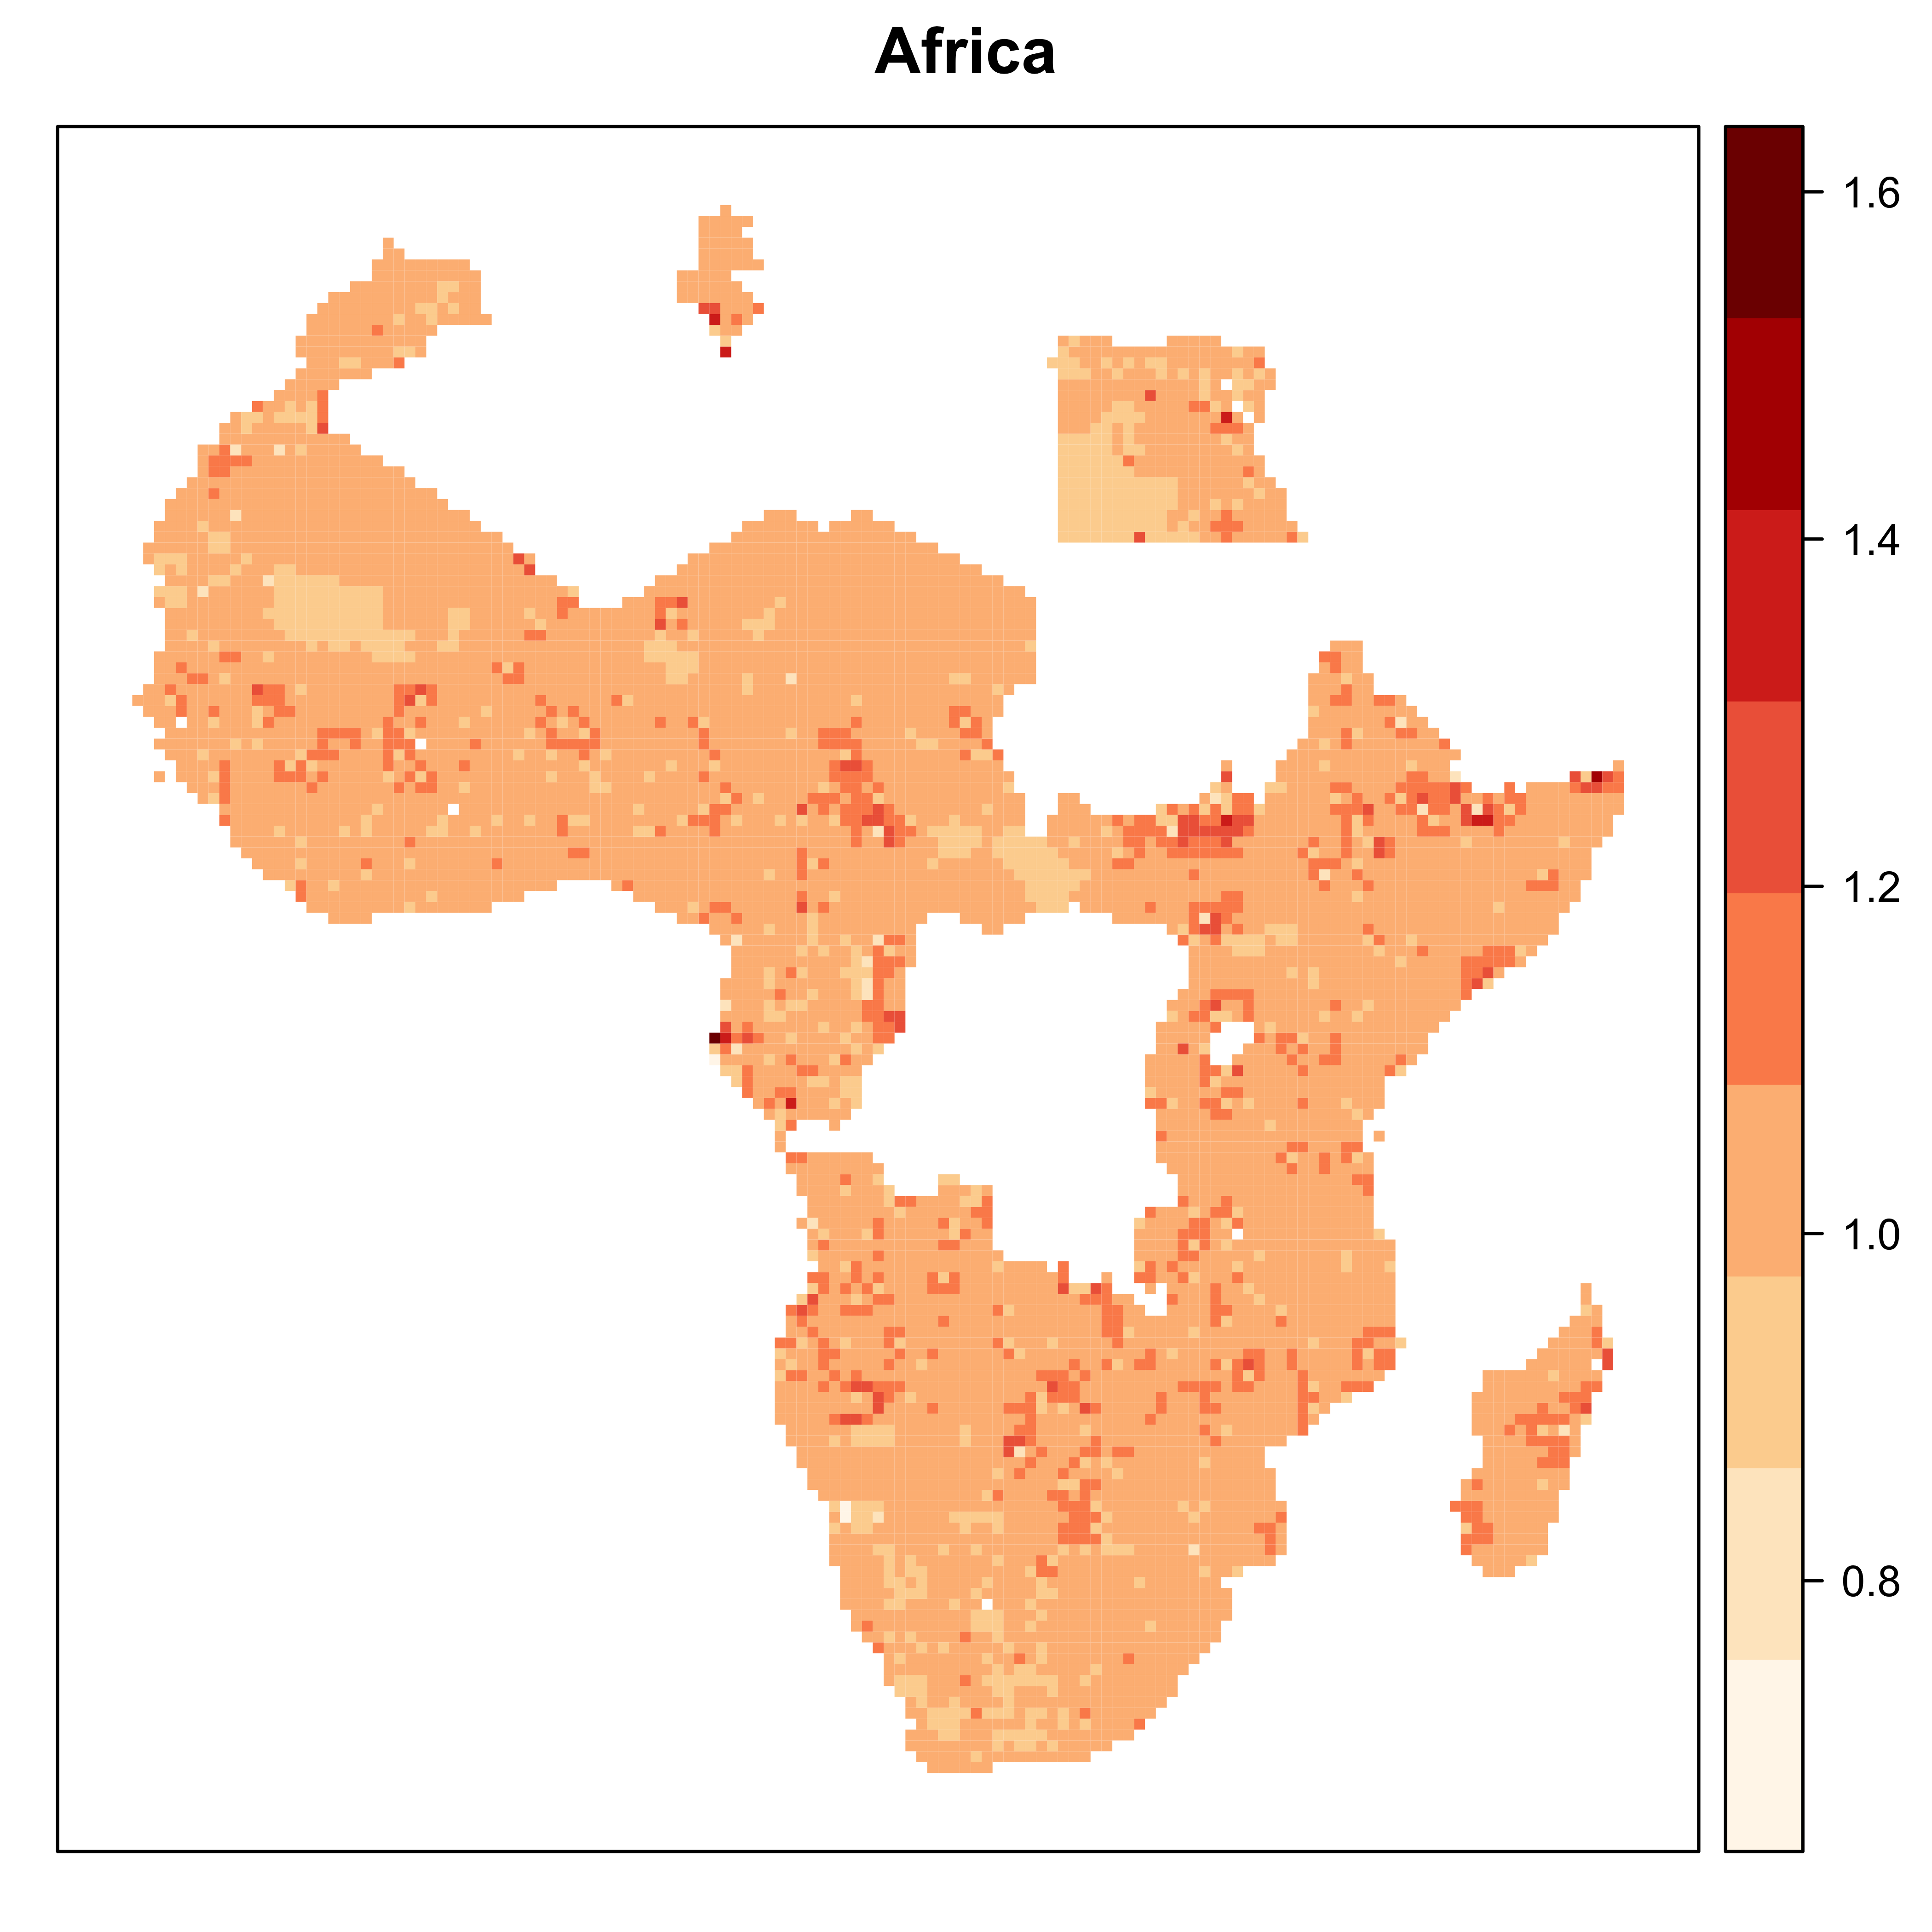
\includegraphics[width=0.65\textwidth,trim={1cm 1cm 1cm 1cm},clip]{/Users/Tilmanski/Documents/UNI/MPhil/Second Year/Thesis_Git/Analysis/output/zeta_heatmaps/African_gridcells_zeta.png}

\label{fig:all_gridcells_by_zeta}
\end{figure}
% End Figure

Figure \ref{fig:all_gridcells_by_zeta}, lastly, displays the spatial variation of $\zeta_{i}$ over all 10,000+ grid cells of the entire African continent. When interpreting this map, note that grid cells are undergoing the reshuffling scenario solely within their respective country. National borders hence play a role and can at times even clearly be inferred from the printed map. Keeping this in mind, the map reveals substantial spatial variation in the infrastructure gap across the African continent. The luckiest region (in Namibia) stands to loose almost 30\% of total welfare if the fictitious social planner intervened and reshuffled roads away from. On the other hand of the spectrum, the residents of one grid cell in Gabon are missing out on a welfare hike of more than 50\%. Moreover, abandoned regions are clearly displaying spatial correlation with large neighbouring swaths of land collectively missing out on infrastructure improvements in certain countries. This begs the conclusion that countries do not just overlook single grid cells but rather live with vast stretches of disadvantaged regions.

In the following section, I proceed to investigate the patterns behind this heterogeneity of network inefficiency over space.
% End Chapter

\section{Results}

% Figure
\begin{table}[] \centering
  \caption{Colonial Railroads and Infrastructure Gap}
  \label{RailKM_zeta}
  \resizebox{\textwidth}{!}{


  \begin{tabular}{@{\extracolsep{5pt}}lcccccccc}
\\[-1.8ex]\hline
\hline \\[-1.8ex]
 & \multicolumn{8}{c}{\textit{Dependent variable:}} \\
\cline{2-9}
\\[-1.8ex] & \multicolumn{8}{c}{Infrastructure Gap $\zeta_{i}$} \\
\\[-1.8ex] & (1) & (2) & (3) & (4) & (5) & (6) & (7) & (8)\\
\hline \\[-1.8ex]
 KM of Colonial Railroads & $-$0.0002$^{***}$ & $-$0.0001$^{***}$ & $-$0.0002$^{***}$ & $-$0.0002$^{***}$ &  &  &  &  \\
  & (0.0001) & (0.0001) & (0.0001) & (0.0001) &  &  &  &  \\
  & & & & & & & & \\
 Km of Colonial Placebo Railroads &  &  &  &  & 0.00004 & $-$0.0002 & $-$0.0003 & $-$0.0003 \\
  &  &  &  &  & (0.0003) & (0.0003) & (0.0003) & (0.0003) \\
  & & & & & & & & \\
\hline \\[-1.8ex]
Country FE &  & Yes & Yes & Yes &  & Yes & Yes & Yes \\
Geographic controls &  &  & Yes & Yes &  &  & Yes & Yes \\
Simulation controls &  &  &  & Yes &  &  &  & Yes \\
Observations & 10,158 & 10,158 & 10,158 & 10,158 & 10,158 & 10,158 & 10,158 & 10,158 \\
R$^{2}$ & 0.001 & 0.099 & 0.111 & 0.113 & 0.00000 & 0.098 & 0.110 & 0.112 \\
\hline
\hline \\[-1.8ex]
\textit{Note:}  & \multicolumn{8}{r}{$^{*}$p$<$0.1; $^{**}$p$<$0.05; $^{***}$p$<$0.01} \\
\end{tabular}

}

\justify
\textit{\\ \footnotesize This table displays results of estimation of equation \ref{eq:regression} on the sample of 0.5x0.5 degree grid cells for the entire African continent (excluding five small countries, see text). Dependent variable is the infrastructure gap for each grid cell. Columns (1)-(4) estimate the effect of colonial infrastructure investments on today's infrastructure gap. Starting with a simple univariate cross-section in (1), column (2) adds 49 country-fixed effects. Column (3) adds geographic controls, consisting of altitude, temperature, average land suitability, malaria prevalence, yearly growing days, average precipitation, and the fourth-order polynomial of latitude and longitude. Simulation controls are added in column (4) and are comprised of population, night lights, ruggedness, and a dummy for whether a cell is classified as urban. These are indicators that went into the original infrastructure re-allocation simulation and are hence not orthogonal to $\zeta$. Columns (5)-(8) repeat these calculations with railroads that were planned, but never built (``placebo railroads''). Results are robust to using only the subsample of 33 countries with any colonial infrastructure investment as reported by \cite{jedwab_permanent_2016}, plus South Africa. Heteroskedasticity-robust standard errors are clustered on the 3x3 degree level and are shown in parantheses.}
\end{table}
% End Figure


% Figure
\begin{table}[] \centering
  \caption{General Equilibrium Effects of Colonial Railroads}
  \label{RailBlocks_zeta}
  \resizebox{\textwidth}{!}{


  \begin{tabular}{@{\extracolsep{5pt}}lcccccccc}
\\[-1.8ex]\hline
\hline \\[-1.8ex]
 & \multicolumn{8}{c}{\textit{Dependent variable: Infrastructure Gap $\zeta$}} \\
\cline{2-9}
\\[-1.8ex] & \multicolumn{6}{c}{Full Sample} &  \multicolumn{2}{c}{Restricted Sample} \\
\\[-1.8ex] & (1) & (2) & (3) & (4) & (5) & (6) & (7) & (8)\\
\hline \\[-1.8ex]
 $<10$ KM to Colonial Railroad & $-$0.013$^{***}$ & $-$0.015$^{***}$ & $-$0.016$^{***}$ &  &  &  & $-$0.014$^{***}$ &  \\
  & (0.003) & (0.004) & (0.004) &  &  &  & (0.004) &  \\
  & & & & & & & & \\
 $10-20$ KM to Colonial Railroad & $-$0.013$^{***}$ & $-$0.015$^{***}$ & $-$0.016$^{***}$ &  &  &  & $-$0.015$^{***}$ &  \\
  & (0.005) & (0.005) & (0.005) &  &  &  & (0.005) &  \\
  & & & & & & & & \\
 $20-30$ KM to Colonial Railroad & $-$0.002 & $-$0.004 & $-$0.005 &  &  &  & $-$0.004 &  \\
  & (0.004) & (0.004) & (0.004) &  &  &  & (0.004) &  \\
  & & & & & & & & \\
 $30-40$ KM to Colonial Railroad & 0.010$^{**}$ & 0.008$^{*}$ & 0.008 &  &  &  & 0.008$^{*}$ &  \\
  & (0.005) & (0.005) & (0.005) &  &  &  & (0.005) &  \\
  & & & & & & & & \\
 $<10$ KM to Colonial Placebo Railroad &  &  &  & $-$0.005 & $-$0.005 & $-$0.006 &  & $-$0.007$^{*}$ \\
  &  &  &  & (0.004) & (0.004) & (0.004) &  & (0.004) \\
  & & & & & & & & \\
 $10-20$ KM to Colonial Placebo Railroad &  &  &  & $-$0.003 & $-$0.004 & $-$0.004 &  & $-$0.004 \\
  &  &  &  & (0.005) & (0.005) & (0.005) &  & (0.005) \\
  & & & & & & & & \\
 $20-30$ KM to Colonial Placebo Railroad &  &  &  & $-$0.001 & $-$0.001 & $-$0.001 &  & $-$0.003 \\
  &  &  &  & (0.004) & (0.004) & (0.004) &  & (0.004) \\
  & & & & & & & & \\
 $30-40$ KM to Colonial Placebo Railroad &  &  &  & 0.007 & 0.006 & 0.005 &  & 0.003 \\
  &  &  &  & (0.004) & (0.004) & (0.004) &  & (0.004) \\
  & & & & & & & & \\
\hline \\[-1.8ex]
Country FE & Yes & Yes & Yes & Yes & Yes & Yes & Yes & Yes \\
Geographic controls &  & Yes & Yes &  & Yes & Yes & Yes & Yes \\
Simulation controls &  &  & Yes &  &  & Yes & Yes & Yes \\
Observations & 10,158 & 10,158 & 10,158 & 10,158 & 10,158 & 10,158 & 6,362 & 6,362 \\
R$^{2}$ & 0.101 & 0.114 & 0.116 & 0.099 & 0.110 & 0.112 & 0.115 & 0.110 \\
\hline
\hline \\[-1.8ex]
\textit{Note:}  & \multicolumn{8}{r}{$^{*}$p$<$0.1; $^{**}$p$<$0.05; $^{***}$p$<$0.01} \\
\end{tabular}

}

\justify
\textit{\\ \footnotesize This table displays effects of various distance-intervals on the infrastructure gap $\zeta$. Explanatory covariates are dummy-variables indicating whether a cell's centroid is within X kilometres to its closest colonial railroad. Geographic controls consist of altitude, temperature, average land suitability, malaria prevalence, yearly growing days, average precipitation, and the fourth-order polynomial of latitude and longitude. Simulation controls are comprised of population, night lights, ruggedness, and a dummy for whether a cell is classified as urban. Columns (1)-(3) examine the effect of actually built colonial railroads. Columns (4)-(6) repeat these calculations with railroads that were planned, but never built (``placebo railroads''). Columns (7)-(8) restrict the sample to the 32 countries on which data for colonial railways is available. Heteroskedasticity-robust standard errors are clustered on the 3x3 degree level and are shown in parantheses.}
\end{table}
% End Figure


% Figure
\begin{table}[] \centering
  \caption{Heterogeneous Effects of Colonial Railroads}
  \label{RailBlocks_mining_military}
  \resizebox{\textwidth}{!}{


  \begin{tabular}{@{\extracolsep{5pt}}lcccccc}
  \\[-1.8ex]\hline
  \hline \\[-1.8ex]
   & \multicolumn{6}{c}{\textit{Dependent variable:}} \\
  \cline{2-7}
  \\[-1.8ex] & \multicolumn{6}{c}{Infrastructure Gap $\zeta$} \\
  \\[-1.8ex] & (1) & (2) & (3) & (4) & (5) & (6)\\
  \hline \\[-1.8ex]
   KM of Colonial Rails for Military Purposes & $-$0.0002$^{***}$ & $-$0.0002$^{***}$ &  &  & $-$0.0002$^{**}$ & $-$0.0002$^{**}$ \\
    & (0.0001) & (0.0001) &  &  & (0.0001) & (0.0001) \\
    & & & & & & \\
   KM of Colonial Rails for Mining Purposes &  &  & $-$0.0001 & $-$0.0001 & $-$0.0001 & $-$0.0001 \\
    &  &  & (0.0001) & (0.0001) & (0.0001) & (0.0001) \\
    & & & & & & \\
  \hline \\[-1.8ex]
  Country FE & Yes & Yes & Yes & Yes & Yes & Yes \\
  Geographic controls & Yes & Yes & Yes & Yes & Yes & Yes \\
  Simulation controls &  & Yes &  & Yes &  & Yes \\
  Observations & 10,158 & 10,158 & 10,158 & 10,158 & 10,158 & 10,158 \\
  R$^{2}$ & 0.110 & 0.112 & 0.110 & 0.112 & 0.110 & 0.113 \\
  \hline
  \hline \\[-1.8ex]
  \textit{Note:}  & \multicolumn{6}{r}{$^{*}$p$<$0.1; $^{**}$p$<$0.05; $^{***}$p$<$0.01} \\
  \end{tabular}

}

\justify
\textit{\\ \footnotesize This table replicated the estimations of Table \ref{RailKM_zeta} in estimating effects of colonial railroads on the infrastructure gap $\zeta$. Colonial rails are classified as built for military or mining purposes (or neither or both) by \cite{jedwab_permanent_2016}. Geographic controls consist of altitude, temperature, average land suitability, malaria prevalence, yearly growing days, average precipitation, and the fourth-order polynomial of latitude and longitude. Simulation controls are comprised of population, night lights, ruggedness, and a dummy for whether a cell is classified as urban. Results are mostly robust for using only the sub-sample of 32 countries for which this data is available, however the p-value of negative impact of military rails increases to $p=0.013$ (Country FE and Geographic Controls) and $p=0.096$ (Country FE, Geographic, and Simulation Controls). Heteroskedasticity-robust standard errors are clustered on the 3x3 degree level and are shown in parantheses.}
\end{table}
% End Figure



%-------------------------------------------------

\newpage
\begin{spacing}{1.0}
\setlength{\bibsep}{2.5pt plus 1.5ex}
\bibliography{Thesis_library}
\end{spacing}

\end{document}
